\section{Continious Integration und Deployment}

Zusätzlich war eine implementation einer Continious Integration, sowie eines Continious Deployments geplant. 
Die beiden Begriffe lassen sich mit CI/CD abkürzen.
Sie sind für eine Automatisierung zuständig während der Softwareentwicklung. 

\subsection{Continious Integration}

Eine Continious Integration bedeutet, dass die Applikationsänderungen mittels mehreren Überprüfungen auf ihre Funktionalität getestet wird.
Dies ist besonders praktikabel, wenn im Projekt mehrere Entwickler Änderungen im Code vornehmen. 
Eine CI Pipeline stellt sicher, dass diese keinen Konflikt verursachen bei der Zusammenführung dieser verschiedener Versionen entsteht. 
Dies geschieht, durch Ausführung des Programms und eine Validierung der Tests. 
\cite{cicdabout}

Solch eine Automatisierung kann durch mehrere Arten verwirklicht werden, wie beispielsweise durch GitHub Actions. 
In jedem GitHub Repository gibt es eine Registerkarte namens \emph{Actions}, diese bietet Vorschläge zur Erstellung solch einer Pipeline (siehe Abb. \ref{fig:implementation:ghactions}). 

\begin{figure}
    \centering
    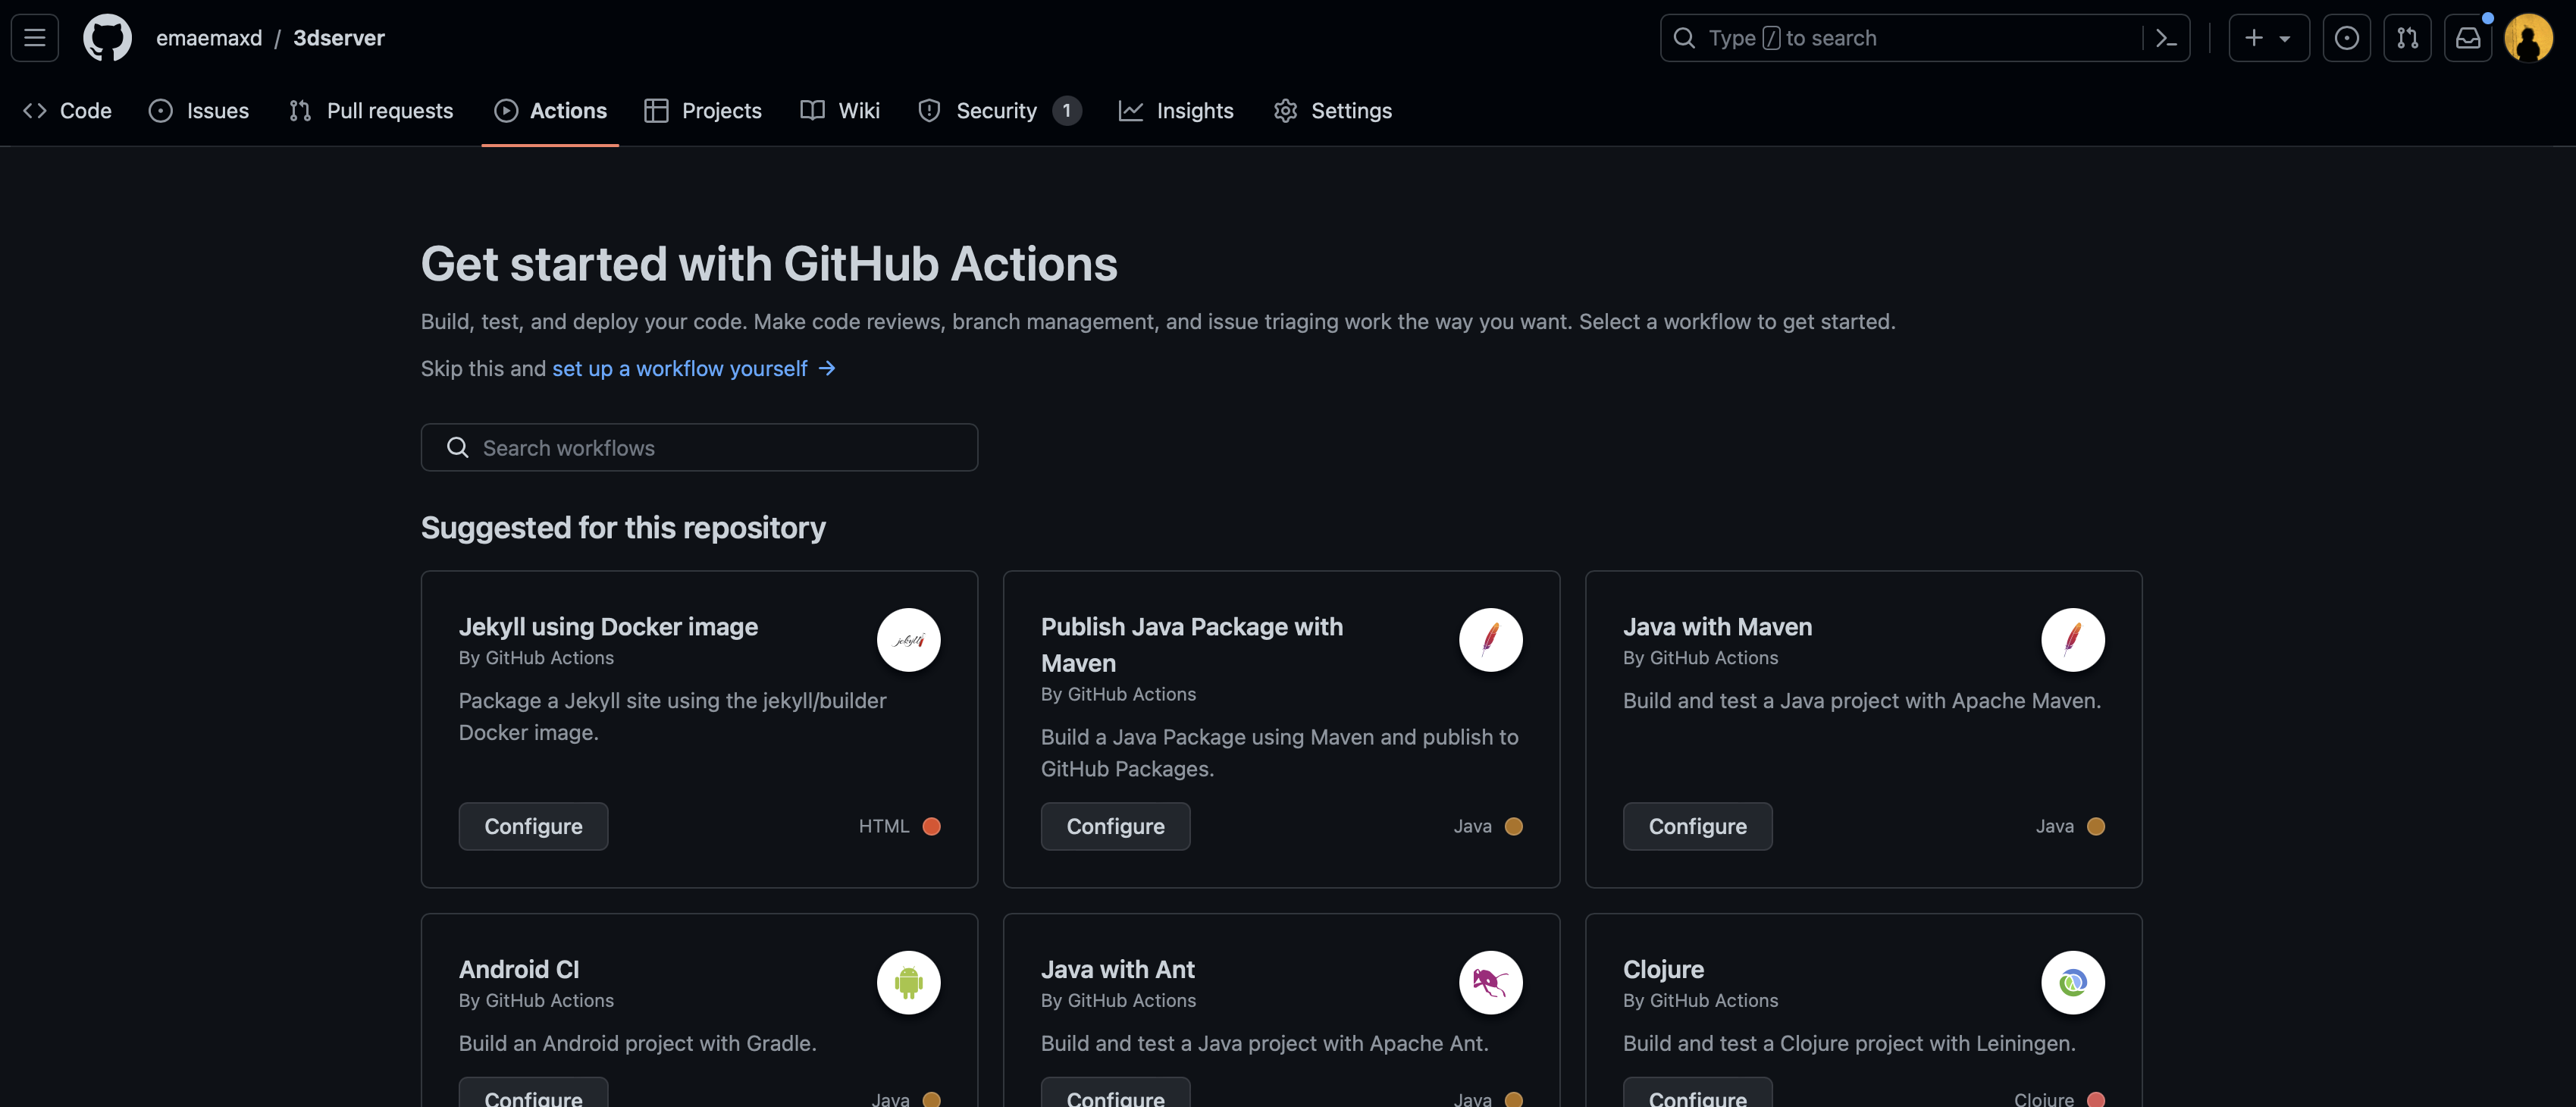
\includegraphics[scale=0.25]{pics/githubactions.png}
    \caption{GitHub Actions Benutzeroberfläche}
    \label{fig:implementation:ghactions}
\end{figure}

Jede Pipeline, oder auch Prozesskette, sind Dateien, welche in einem Ordner namens \emph{workflows} angelegt werden. 
In diesen Dateien sind Prozesse und Konfigurationen definiert, wie beispielsweise der Name der Pipeline.
Ebenso wird definiert, wann diese ausgeführt werden. 
Im Codeausschnitt \ref{lst:cipipeline} in Zeile 3 bis 7 wurde definiert, dass die nachfolgenden Steps bei jedem Push- und Pull-Request am Main Branch ausgeführt werden. 
Ebenso wird der benötigte Runner definiert in Zeile 11. 
Danach werden die einzelnen Schritte definiert, um die \gls{ci} für die Applikation zu erstellen, zum Beispiel die Installation aller node Module. 
In diesem Fall sind alle Steps Teil von einem einzigen Job namens "build". 

\begin{lstlisting}[label=lst:cipipeline, language=bash, caption=Pipeline einer CI]
name: CI

on:
  push:
    branches: [ main ]
  pull_request:
    branches: [ main ]
  # ...
jobs:
  build:
    runs-on: ubuntu-latest

    steps:
      - uses: actions/checkout@v2

      - name: Install all node modules
        run: npm i 
        working-directory: ./3D-Portfolio-Gallery/
    # ...

\end{lstlisting}

\subsection{Continious Delivery}

Eine \gls{cd} ist sozusagen der ein Upgrade der \gls{ci}. 
Das Ziel dieser ist es, die Applikation für die Produktion bereitzustellen. 
Dies geschieht ebenfalls durch eine Pipeline, welche die Anwendung Schritt für Schritt durchtestet und anschließend auf den Produktionsserver lädt. 
\cite{cicdabout}

Während der Entwicklung kam es zu dem Fazit, dass eine Konfiguration einer CI/CD Pipeline als nicht nötig empfunden wurde. 
Dies ist einerseits, da nur eine Person an dem Backend arbeitete und somit keine zweite Validierung der Software nötig war, da diese schon manuell ausgeführt wurden. 
Andererseits hätte es eine große Komplexität bedeutet, da Frontend und Backend auf unterschiedlichen Repositories entwickelt wurden. 
 